\documentclass{beamer}
\mode<presentation>
{
  \usetheme{default}      % or try Darmstadt, Madrid, Warsaw, ...
  \usecolortheme{default} % or try albatross, beaver, crane, ...
  \usefonttheme{default}  % or try serif, structurebold, ...
  \setbeamertemplate{navigation symbols}{}
  \setbeamertemplate{caption}[numbered]
} 

\usepackage[english]{babel}
\usepackage[utf8x]{inputenc}
\usepackage{scrextend}
\usepackage{graphicx}
\usepackage{booktabs}
\usepackage{adjustbox}
\usepackage{marvosym}
\graphicspath{ {E:/faculta/Master/DissertationProject/images/} }

\title[Pres]{Dezvoltarea de metode de analiza automata a sistemelor software}
\author{Stana Adelina Diana}
\institute{Computer Science and Engineering Department\\
"Politehnica" University of Timisoara}
\date{Iulie, 2018}

\begin{document}

\begin{frame}
  \titlepage
\end{frame}

% Uncomment these lines for an automatically generated outline.
%\begin{frame}{Outline}
%  \tableofcontents
%\end{frame}

%%%%%%%%%%%%%%%%%%%%%%%%%%%%%%%%%%%%%%%%%%

 \begin{frame}
\frametitle{Pregătirea anterioară}
\begin{block}{}
Întreaga pregătire anterioară a fost pe direcția de Inginerie Software din cadrul domeniului Calculatoare și Tehnologia Informației, fiind în concordanță deplină cu domeniul de doctorat.
\end{block}

Studiile absolvite pană in prezent sunt:\\
- \textbf{Licența} la facultatea de Automatică și Calculatoare, UPT, in domeniul Calculatoare și Tehnologia Informației, specializarea Calculatoare, cu opționale pe pachetul de Software Engineering, media de absolvire 8,87.

Tema lucrarii de licenta a fost \textit{“Sistem distribuit pentru gestionarea interacțiunii clienților cu sistemul de versionare.”} obtinând nota 9,66  în sesiunea Iunie 2016.

\end{frame}

%%%%%%%%%%%%%%%%%%%%%%%%%%%%%%%%%%%%%%%%%%

 \begin{frame}
\frametitle{Pregătirea anterioară}

- \textbf{Master} la facultatea de Automatică și Calculatoare, UPT, in domeniul Calculatoare și Tehnologia Informației, specializarea Information Technology, media de absolvire 9,75. 

Tema lucrarii de dizertatie a fost \textit{“An analysis of the relationship between structural and logical dependencies in software systems.”} obtinând nota 10 în sesiunea Iunie 2018.

\end{frame}


%%%%%%%%%%%%%%%%%%%%%%%%%%%%%%%%%%%%%%%%%%%

 \begin{frame}
\frametitle{Gradul de inițiere în activități de cercetare}
\begin{block}{}
În cadrul departamentului de Calculatoare cu ocazia elaborării lucrării de dizertație. 
\end{block}

Lucrarea de disertație a avut ca obiectiv principal studiul relațiilor dintre diferitele tipuri de dependențe software: dependențe structurale, extrase din analiză statică a codului sursă, și dependențe logice, extrase din modul de evoluție al sistemului regăsit  în sistemul de versionare. 
\end{frame}

%%%%%%%%%%%%%%%%%%%%%%%%%%%%%%%%%%%%%%%%%%%

 \begin{frame}
\frametitle{Gradul de inițiere în activități de cercetare }
Pentru aceasta, am construit un tool de analiză pentru extragerea ambelor tipuri de dependențe software. 
\begin{center}
     \begin{figure}
	\includegraphics[width=\textwidth]{tool2.png}
	\caption{\label{fig:figtool} User Interface}
     \end{figure}
\end{center}

\end{frame}

%%%%%%%%%%%%%%%%%%%%%%%%%%%%%%%%%%%%%%%%%%%

 \begin{frame}
\frametitle{Gradul de inițiere în activități de cercetare}
tbd
\begin{center}
     \begin{figure}
	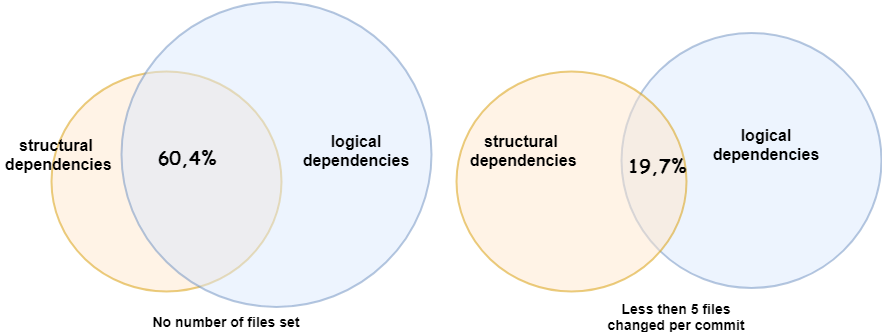
\includegraphics[width=\textwidth]{fig4.png}
	\caption{\label{fig:figtool} Rezultate}
     \end{figure}
\end{center}

\end{frame}

%%%%%%%%%%%%%%%%%%%%%%%%%%%%%%%%%%%%%%%%%%
 \begin{frame}
\frametitle{Direcțiile și intențiile de studiu avute în vedere pentru programul doctoral}
Tema aleasa este "Dezvoltarea de metode de analiza automata a sistemelor software" din oferta doctorala a prof.dr.ing. Vladimir Cretu și constă în dezvoltarea de metode și tehnici automate de analiza a sistemelor software, aducând contribuții noi prin valorificarea informațiilor referitoare la modul de evoluție a sistemelor analizate, obținute din sistemele de versionare. 

\end{frame}

%%%%%%%%%%%%%%%%%%%%%%%%%%%%%%%%%%%%%%%%%%%

 \begin{frame}
\frametitle{Lucrări stiințifice}
[1] Adelina Stana, Ioana Șora, \textit{„An analysis of the relationship between structural and logical dependencies in software systems”} trimisă la Sesiunea de Comunicări Ştiinţifice Studenţeşti UPT, comunicată.


[2] Adelina Stana, Ioana Șora, Vladimir Crețu, \textit{„Logical dependencies between classes: how to find them and how to use them ?”} trimisă la The 34th IEEE International Conference on Software Maintenance and Evolution (ICSME) 2018 - Doctoral Symposium, Madrid, Spania, Sept 2018, lucrare acceptată.
\end{frame}

%%%%%%%%%%%%%%%%%%%%%%%%%%%%%%%%%%%%%%%%%%%

 \begin{frame}
\frametitle{Lucrări stiințifice}
[3] Ioana Șora, Adelina Stana, \textit{„Identifying logical dependencies from co-changing classes”}  trimisă la The 7th International Workshop on Mining Software Repositories (SOFTWAREMINING-2018) - colocated with The 33rd IEEE/ACM International  Conference on Automated Software Engineering (ASE 2018), Montpellier, Franta, Sept 2018, în așteptarea deciziei de review.
\end{frame}



%%%%%%%%%%%%%%%%%%%%%%%%%%%%%%%%%%%%%%%%%%%

\end{document}
